%&bericht

%%%%%%%%%%%%%%%%%%%%%%%%%%%%%%%%%%%%%%%%%%%%%%%%%%%%%%%%%%%%%%%%%%%%%%%%%%%%%%%
%% Descr:       Vorlage für Berichte der DHBW-Karlsruhe
%% Author:      Prof. Dr. Jürgen Vollmer, juergen.vollmer@dhbw-karlsruhe.de
%% $Id: bericht.tex,v 1.25 2020/03/13 15:07:45 vollmer Exp $
%%  -*- coding: utf-8 -*-
%%%%%%%%%%%%%%%%%%%%%%%%%%%%%%%%%%%%%%%%%%%%%%%%%%%%%%%%%%%%%%%%%%%%%%%%%%%%%%%

\documentclass[
   ngerman          % neue deutsche Rechtschreibung
  ,a4paper          % Papiergrösse
% ,twoside          % Zweiseitiger Druck (rechts/links)
% ,10pt             % Schriftgrösse
  ,11pt
% ,12pt
  ,pdftex
%  ,disable         % Todo-Markierungen auschalten
]{report}

% Bitte die Codierung Ihrer Dateien auswählen:
% \usepackage[latin1]{inputenc}    % Für UNIX mit ISO-LATIN-codierten Dateien
% \usepackage[applemac]{inputenc}  % Für Apple Mac
% \usepackage[ansinew]{inputenc}   % Für Microsoft Windows
\usepackage[utf8]{inputenc}        % UTF-8 codierte Dateien
                                   % Dieses Dokument ist unter Unix erstellt, daher
                                   % wird diese Input-Codierung benutzt.

\usepackage{bericht}
\usepackage[graphicx]{realboxes}
%\usepackage[landscape]{geometry}
\usepackage{lscape}

%% ACHTUNG, wenn man eine eigene Formatdatei (bericht.fmt) benutzt, werden Änderungen an bericht.sty
%% erst wirksam, wenn die Format-Datei neu erzeugt wurde!!!
%% Genauer alle Änderungen, die textuell vor der nächsten Zeile ".... endofdump...." stehen
%% werden erst wirksam, wenn die Formatdatei neu erzeugt wurde
\csname endofdump\endcsname

%%%%%%%%%%%%%%%%%%%%%%%%%%%%%%%%%%%%%%%%%%%%%%%%%%%%%%%%%%%%%%%%%%%%%%%%%%%%%%%
%% Angaben zur Arbeit
%%%%%%%%%%%%%%%%%%%%%%%%%%%%%%%%%%%%%%%%%%%%%%%%%%%%%%%%%%%%%%%%%%%%%%%%%%%%%%%


\newcommand{\Autor}{Lorenz Scherrer}
\newcommand{\MatrikelNummer}{8809469}
\newcommand{\Kursbezeichnung}{tinf21b3}

\newcommand{\FirmenName}{SICK AG}
\newcommand{\FirmenStadt}{Waldkirch}
\newcommand{\FirmenLogoDeckblatt}{\fbox{
\includegraphics[width=3cm]{images/SICK_Logo_Claim}}}

% Falls es kein Firmenlogo gibt:
%  \newcommand{\FirmenLogoDeckblatt}{}

\newcommand{\BetreuerFirma}{Manfred Haberer}
\newcommand{\BetreuerDHBW}{Prof. Dr. Jürgen Vollmer}

%%%%%%%%%%%%%%%%%%%%%%%%%%%%%%%%%%%%%%%%%%%%%%%%%%%%%%%%%%%%%%%%%%%%%%%%%%%%%%%%%%%%%

% Wird auf dem Deckblatt und in der Erklärung benutzt:
\newcommand{\Was}{Projektarbeit}
%\newcommand{\Was}{Projektrarbeit}
%\newcommand{\Was}{Studienarbeit}
%\newcommand{\Was}{Bachleorarbeit}

%%%%%%%%%%%%%%%%%%%%%%%%%%%%%%%%%%%%%%%%%%%%%%%%%%%%%%%%%%%%%%%%%%%%%%%%%%%%%%%%%%%%%

\newcommand{\Titel}{Aufbau und Inbetriebnahme einer virtuellen Applikationsszene für AGVs in Unity}
\newcommand{\AbgabeDatum}{24. September 2023}

\newcommand{\Dauer}{12 Wochen}

% \newcommand{\Abschluss}{Bachelor of Engineering}
\newcommand{\Abschluss}{Bachelor of Science}

\newcommand{\Studiengang}{Informationstechnik}
% \newcommand{\Studiengang}{Informatik / Angewandte Informatik}

\hypersetup{%%
  pdfauthor={\Autor},
  pdftitle={\Titel},
  pdfsubject={\Was}
}

%%%%%%%%%%%%%%%%%%%%%%%%%%%%%%%%%%%%%%%%%%%%%%%%%%%%%%%%%%%%%%%%%%%%%%%%%%%%%%%


% Benutzt man das "biblatex"-Paket, dann muß das hier stehen:
% siehe auch die mit BIBLATEX markierten Zeilen in bericht.sty
\bibliography{bericht}

%\setlength{\marginparwidth}{2cm}

\begin{document}

%%%%%%%%%%%%%%%%%%%%%%%%%%%%%%%%%%%%%%%%%%%%%%%%%%%%%%%%%%%%%%%%%%%%%%%%%%%%%%%

\begin{titlepage}
\begin{center}
\vspace*{-2cm}
\FirmenLogoDeckblatt\hfill
\includegraphics[width=4cm]{images/dhbw-logo}\\[2cm]
{\Huge \Titel}\\[1cm]
{\Huge\scshape \Was}\\[1cm]
{\large für die Prüfung zum}\\[0.5cm]
{\Large \Abschluss}\\[0.5cm]
{\large des Studienganges \Studiengang}\\[0.5cm]
{\large an der}\\[0.5cm]
{\large Dualen Hochschule Baden-Württemberg Karlsruhe}\\[0.5cm]
{\large von}\\[0.5cm]
{\large\bfseries \Autor}\\[1cm]
{\large Abgabedatum \AbgabeDatum}
\vfill
\end{center}
\begin{tabular}{l@{\hspace{2cm}}l}
Bearbeitungszeitraum	          & \Dauer 			        \\
Matrikelnummer	                & \MatrikelNummer		  \\
Kurs			                      & \Kursbezeichnung		\\
Ausbildungsfirma	              & \FirmenName			    \\
			                          & \FirmenStadt			  \\
Betreuer der Ausbildungsfirma	  & \BetreuerFirma		  \\
Gutachter der Studienakademie	  & \BetreuerDHBW		    \\
\end{tabular}
\end{titlepage}

%%%%%%%%%%%%%%%%%%%%%%%%%%%%%%%%%%%%%%%%%%%%%%%%%%%%%%%%%%%%%%%%%%%%%%%%%%%%%%%

%%%%%%%%%%%%%%%%%%%%%%%%%%%%%%%%%%%%%%%%%%%%%%%%%%%%%%%%%%%%%%%%%%%%%%%%%%%%%%%
%% Descr:       Vorlage für Berichte der DHBW-Karlsruhe, Erklärung
%% Author:      Prof. Dr. Jürgen Vollmer, vollmer@dhbw-karlsruhe.de
%% $Id: erklaerung.tex,v 1.11 2020/03/13 14:24:42 vollmer Exp $
%% -*- coding: utf-8 -*-
%%%%%%%%%%%%%%%%%%%%%%%%%%%%%%%%%%%%%%%%%%%%%%%%%%%%%%%%%%%%%%%%%%%%%%%%%%%%%%%

% In Bachelorarbeiten muss eine schriftliche Erklärung abgegeben werden.
% Hierin bestätigen die Studierenden, dass die Bachelorarbeit, etc.
% selbständig verfasst und sämtliche Quellen und Hilfsmittel angegeben sind. Diese Erklärung
% bildet das zweite Blatt der Arbeit. Der Text dieser Erklärung muss auf einer separaten Seite
% wie unten angegeben lauten.

\newpage
\thispagestyle{empty}
\begin{framed}
\begin{center}
\Large\bfseries Erklärung
\end{center}
\medskip
\noindent
% siehe §5(3) der \enquote{Studien- und Prüfungsordnung DHBW Technik} vom 29.\,9.\,2017 und Anhang 1.1.13
Ich versichere hiermit, dass ich meine \Was mit dem Thema:
\enquote{\Titel}
selbstständig verfasst und keine anderen als die angegebenen Quellen und Hilfsmittel benutzt habe. Ich versichere zudem, dass die eingereichte elektronische Fassung mit der gedruckten Fassung übereinstimmt.
\vspace{3cm}
\noindent
\underline{\hspace{4cm}}\hfill\underline{\hspace{6cm}}\\
Ort~~~~~Datum\hfill Unterschrift\hspace{4cm}
\end{framed}

\vfill
\emph{Sofern  vom Dualen Partner ein Sperrvermerk gewünscht wird, ist folgende Formulierung
zu verwenden:}
\begin{framed}
\begin{center}
\Large\bfseries Sperrvermerk
\end{center}
\medskip
\noindent
Der Inhalt dieser Arbeit darf weder als Ganzes noch in Auszügen Personen
außerhalb des Prüfungsprozesses und des Evaluationsverfahrens zugänglich gemacht
werden, sofern keine anderslautende Genehmigung vom Dualen Partner vorliegt.
\end{framed}

%%%%%%%%%%%%%%%%%%%%%%%%%%%%%%%%%%%%%%%%%%%%%%%%%%%%%%%%%%%%%%%%%%%%%%%%%%%%%%%
\endinput
%%%%%%%%%%%%%%%%%%%%%%%%%%%%%%%%%%%%%%%%%%%%%%%%%%%%%%%%%%%%%%%%%%%%%%%%%%%%%%%


%%%%%%%%%%%%%%%%%%%%%%%%%%%%%%%%%%%%%%%%%%%%%%%%%%%%%%%%%%%%%%%%%%%%%%%%%%%%%%%

\newpage
\pagenumbering{Roman}
\tableofcontents           % Inhaltsverzeichnis hier ausgeben
\listoffigures             % Liste der Abbildungen
\listoftables              % Liste der Tabellen
\lstlistoflistings         % Liste der Listings
\listofequations           % Liste der Formeln

% Jetzt kommt der "eigentliche" Text
%%%%%%%%%%%%%%%%%%%%%%%%%%%%%%%%%%%%%%%%%%%%%%%%%%%%%%%%%%%%%%%%%%%%%%%%%%%%%%
%% Descr:       Vorlage für Berichte der DHBW-Karlsruhe, Datei mit Abkürzungen
%% Author:      Prof. Dr. Jürgen Vollmer, vollmer@dhbw-karlsruhe.de
%% $Id: abk.tex,v 1.4 2017/10/06 14:02:03 vollmer Exp $
%% -*- coding: utf-8 -*-
%%%%%%%%%%%%%%%%%%%%%%%%%%%%%%%%%%%%%%%%%%%%%%%%%%%%%%%%%%%%%%%%%%%%%%%%%%%%%%%

\chapter*{Abkürzungsverzeichnis}                   % chapter*{..} -->   keine Nummer, kein "Kapitel"
						         % Nicht ins Inhaltsverzeichnis
% \addcontentsline{toc}{chapter}{Akürzungsverzeichnis}   % Damit das doch ins Inhaltsverzeichnis kommt

% Hier werden die Abkürzungen definiert
\begin{acronym}[DHBW]
  % \acro{Name}{Darstellung der Abkürzung}{Langform der Abkürzung}
 \acro{Abk}[Abk.]{Abkürzung}

 % Folgendes benutzen, wenn der Plural einer Abk. benöigt wird
 % \newacroplural{Name}{Darstellung der Abkürzung}{Langform der Abkürzung}
 \newacroplural{Abk}[Abk-en]{Abkürzungen}

 \acro{H2O}[\ensuremath{H_2O}]{Di-Hydrogen-Monoxid}

 % Wenn neicht benutzt, erscheint diese Abk. nicht in der Liste
 \acro{NUA}{Not Used Acronym}
\end{acronym}
              % Abkürzungsverzeichnis
\newpage

\newcounter{savepage}
\setcounter{savepage}{\value{page}}
\pagenumbering{arabic}

%\chapter{Einleitung}
%Beschreibe den Hintergrund und die Motivation deiner Arbeit. Erkläre, warum dieses Thema wichtig ist und welche Forschungsfragen du untersuchst.
Das Ziel dieser Abreit ist es ein virtuelle Umgebung zu erstellen um für die Entwicklung von Algorithmen für die sichere Personenerkennung in Automated Guided Vehicle. 
%Verstehe das Problem
Es sollen Umweltdaten von Automated Guided Vehicle Applikationen zur Entwicklung generiert werden. Die Umweltdaten sollen zum testen und Validieren von Sicherheitskonzepten. So sollen Worst-Case-Szenarien definiert werden und die Robustheit der Softwarealgorithemen geprüft werden.\\

Der Vorteil ist es das so viele mehr testdaten generiert werden könne ohne aufwendige Test Scenerien in einer realen Werkshalle aufzubauen.\\
%Identifiziere das Problem
%Hintergrundinformationen
%Relavanz betonen
%Ziele und Hypothesen
%Betonung des Neuigkeitswertes
%Zusammenfassung
%Zusätliche Quellen

%\section{Projektumfeld und Kontext}% kann auch weg gelassen werden
%GICTICIISM
%Global Industry Centers Technical Industry Competence \& Innovation

\section{Problemstellung}
%Verständnis des Themas: Stelle sicher, dass du ein klares Verständnis für das Thema deiner Arbeit hast, bevor du die Problemstellung formulierst.
%Identifikation des Problems: Überlege, welche spezifische Frage oder Herausforderung du in deiner Arbeit angehen möchtest. Welche Lücke in der bestehenden Forschung möchtest du schließen oder welches Problem möchtest du lösen?
%DSM Project was ist dieses Projekt?
Die Problemstellung bindet sich im DSM ein. Es sollen die Sceneie aufgebaut werden und die Sensordaten dem gRPC Server bereitgestellten werden.
\begin{figure}[htp]
    \centering
    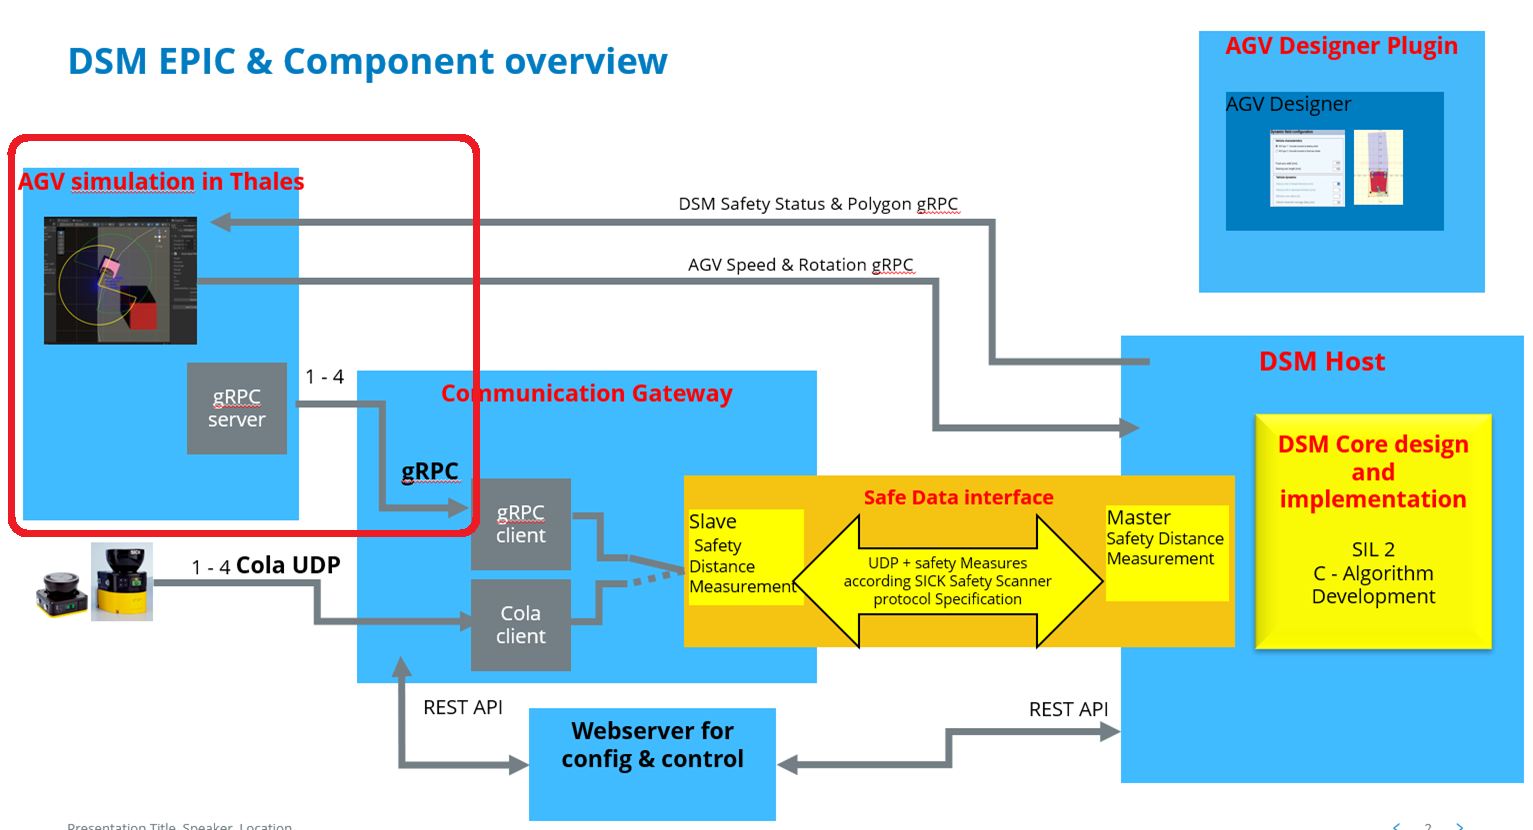
\includegraphics[width=(\textwidth)]{images/AGV_Overview.png}
    \caption{DSM EPIC \& Component overview}
    \label{fig:DSMoverview}
\end{figure}
%Wo finde ich informationen zum DSM Projekt? Boris morgen fragen
%Was trage ich zu deisem Projekt bei?

%Identifiziere die Lücke im Wissen:
Es gib keine Simulation in der man Gefahrensitzuationen testen kann. Ohne Sie in echten Hallen zu testen.
%Spezifische Fragestellung: Formuliere deine Problemstellung als eine klare Frage. Diese Frage sollte präzise, klar und relevant sein. Vermeide vage oder mehrdeutige Formulierungen.


%Bedeutung und Relevanz Betone die Bedeutung deiner Problemstellung. Warum ist es wichtig, diese Frage zu beantworten oder dieses Problem zu lösen? Welche Auswirkungen könnte die Antwort haben?
Im weiteren verlauf kann der Algorithmus der die Sicherheitsfelder der AGVs berechnet an ein Instutut geschickt werden der diesen Valiediert. Oder ein in der Simulation getesten Algorithmus in echten Szenarien getestet werden.
Hier können die Sicherheitsalghrutmen erstmals getestet werden.

%Abgrenzung und Kontext: Kläre den Rahmen deiner Problemstellung. Welche Aspekte deines Themas wirst du behandeln und welche wirst du bewusst außer Acht lassen? Definiere den Kontext, in dem deine Fragestellung relevant ist.


\section{Zielsetzung}
%Die Zielsetzung beschreibt das übergeordnete Ziel deiner Arbeit. Sie verdeutlicht, was du mit deiner Forschung erreichen möchtest.
%Konkretheit: Formuliere deine Zielsetzung so konkret wie möglich. Vermeide allgemeine Formulierungen, die mehrdeutig sind.
%Messbarkeit: Stelle sicher, dass dein Ziel messbar ist. Das bedeutet, dass du später überprüfen können solltest, ob du es erreicht hast.
%Realistisch: Deine Zielsetzung sollte realistisch sein und in einem angemessenen Rahmen erreichbar sein.
%Relevanz: Betone, warum dein Ziel wichtig ist und welche Bedeutung es für die Forschung oder die Praxis hat.
Daten übermittel und ein AGv in Unity erstellen.

\section{Fragestellung}
%Die Forschungsfrage konkretisiert deine Zielsetzung und gibt die Richtung für deine Untersuchung vor. Sie sollte präzise, klar und offen genug sein, um die Möglichkeit zur Forschung zu bieten.
%Klarheit: Formuliere die Forschungsfrage klar und verständlich. Vermeide komplexe Satzstrukturen.
%Ein Frageaspekt: Fokussiere auf einen bestimmten Aspekt des Themas. Eine zu breite Fragestellung kann zu unübersichtlichen Ergebnissen führen.
%Beantwortbarkeit: Stelle sicher, dass deine Forschungsfrage durch deine Forschungsmethoden und Daten beantwortbar ist.

Wie kann ein AGV in Unity in erstellt werden und dessen Meschanische Daten über gRPC mit der Ausenwelt geteilt werden und auch Daten erhalten? 
%\section{Zeitplan}
\subsection{Projektstrukturplan}
\begin{figure}[h]
 \centering
 \includegraphics{input/Strukturplan.drwio.png}
 \caption{Meine Grafik}
 \label{fig:meine-grafik}
\end{figure}
Mit Draw.io machen
\subsection{Zielvorgaben}
\subsection{Begenzte Ressourcen}
\begin{itemize}
    \item 13. Juli - 21. Juli = 7 Tage
    \item 4. September - 30. September = 20 Tage
    \item 27 Arbeitstage a 7 Stunden gleich 189 Stunden
\end{itemize}


%\include{input/Riskomodelle}
%\chapter{Implementierung}
\section{Implementierung der Schnittstelle}
\section{AGVs in der virtuellen Umgebung}
%\include{input/schlussbetrachtung}
\section{Notizen}
\subsection{Aufgaben}
Die Aufgabe ist es sich in Unity ein zuarbeiten. Dort eine Scenerie aufzubauen und die Daten die die vier Sensoren liefern mit den Bewegungs vektoren übertragen.
Die übertragung soll über einen gRPC Client und einen gRPC Server laufen. Dannach sollen mit den erzeugten Daten das Feld des DSM Host in Unity angezeigt werden(Best Case für Demo gedacht).
\begin{itemize}
    \item Zeitplan
    \item Riskomanagment
    \item 
\end{itemize}
\subsection{Zeitplan}

\begin{itemize}
    \item 13. Juli - 21. Juli = 7 Tage
    \item 4. September - 30. September = 20 Tage
    \item 27 Arbeitstage a 7 Stunden gleich 189 Stunden
\end{itemize}



% Please add the following required packages to your document preamble:
% \usepackage[table,xcdraw]{xcolor}
% If you use beamer only pass "xcolor=table" option, i.e. \documentclass[xcolor=table]{beamer}

\begin{landscape}
    
\begin{tabularx}{21cm}{|l|l|l|X|X|X|X|X|X|X|X|X|X|X|X|}
    \hline
    \textbf{Aufgabe}                       & \textbf{Anfang} & \textbf{Ende} & \textbf{28}            & \textbf{29}            & \textbf{30}            & \textbf{31}            & \textbf{32}            & \textbf{33}            & \textbf{34}            & \textbf{35}            & \textbf{36}            & \textbf{37}            & \textbf{38}            & \textbf{39}            \\ \hline
    Planung+ Aufgabe Prio 1                & 12.07           & 14.07         & \cellcolor[HTML]{34CDF9} &                          &                          &                          &                          &                          &                          &                          &                          &                          &                          &                          \\ \hline
    Aufgabe Prio 2                         & 17.07           & 21.07         &                          & \cellcolor[HTML]{34CDF9} &                          &                          &                          &                          &                          &                          &                          &                          &                          &                          \\ \hline
    Abwesenheit                            & 24.07           & 01.09         &                          &                          & \cellcolor[HTML]{C0C0C0} & \cellcolor[HTML]{C0C0C0} & \cellcolor[HTML]{C0C0C0} & \cellcolor[HTML]{C0C0C0} & \cellcolor[HTML]{C0C0C0} & \cellcolor[HTML]{C0C0C0} &                          &                          &                          &                          \\ \hline
    Aufgabe Prio 2                         & 04.09           & 08.09         &                          &                          &                          &                          &                          &                          &                          &                          & \cellcolor[HTML]{34CDF9} &                          &                          &                          \\ \hline
    Aufgabe Prio 3                         & 11.09           & 15.09         &                          &                          &                          &                          &                          &                          &                          &                          &                          & \cellcolor[HTML]{34CDF9} &                          &                          \\ \hline
    Aufgabe Prio 4+Doku                    & 18.09           & 29.09         &                          &                          &                          &                          &                          &                          &                          &                          &                          & \cellcolor[HTML]{68CBD0} & \cellcolor[HTML]{68CBD0} & \cellcolor[HTML]{68CBD0} \\ \hline
    Praxisbericht + Kollogium Vorbereitung & 18.09           & 22.09         &                          &                          &                          &                          &                          &                          &                          &                          &                          &                          & \cellcolor[HTML]{34FF34} &                          \\ \hline
    Kollogium                              & 25.09           & 29.09         &                          &                          &                          &                          &                          &                          &                          &                          &                          &                          &                          & \cellcolor[HTML]{FE0000} \\ \hline
\end{tabularx}
\end{landscape}
   

\subsection{Notizen 03.07}
Unity zum laufen bekommen auf dem anderen PC.


\subsection{Themenbesprechung Protokoll}
Welche Scenarian sind reelevant?
Vergleich zwischen Unity und Ross
Zeitplan erstellen
Aufgabenpakte erstellen
Riskomodelle
Riskoeinschätzung
Was kann schief gehen?
EIn kapitel Riskomanament
Ein kapitel Zeitplan Arbietspakete
Problemstellung verstehen
Schutzfelder nicht
ein zwei Wochen Arbeitspakete
Wochen Meeting
Jira nach Zeitplan füllen
Zeit ein planen zum Bericht schreiben jeden Tag eine Stunde 


Prios der arbeit
Prio 1 Senordaten über gRPC übertragen
Prio 2 Wenderadius und Geschwindigkeit übertragen mit der Thales (Einauto selbst Desginen)
es gibt mehrer auto: gabelstapler, Panzerrolle, normale Auto
Prio 3 Polghonzug erhalten und in Unity darstellen
Prio 4 NotSignal erhalten und das AGV anhalten 
Prio 5 Beispiel Scene zu Sever Client wo die Daten von einem Sensor übertragen werden. Dann auch noch die Parameter von einem Template GameObject übertragen wird.


\subsection{12.07}
Plan für heute dem AGV Geschwindigkeit geben. Und weiter geben. Das Problem die AGV/Service wird nicht erkannt. Obwohl der SplineWalker mit dem dem Agv Service Script verbunden ist. Die 

\subsection{13.07}
\begin{itemize}
\item Projekt Einsicht in VS Studio
\item Martin schreiben wegen dem AGV übertragung
\item Fragen formulieren zur Thales Schnittstelle
\item 
\end{itemize}

Fragen zur Thales Schnittstelle
\begin{itemize}
\item Jan hat eine Agvservice script erstellt welches IAgv verwendet aber es wird nicht bei den Avalibele Services angezeigt
\item Hallo Martin wir haben noch ein paar Fragen zur Thales Api. Hast du heute Nachmittag Zeit für ein Meeting mit Artem und mir?
\end{itemize}

\subsection{14.07}
\begin{itemize}
\item Sprint Meeting vorbereiten
\item die vier Scanner abfragen und übertragen. Wie funktioiert das mit dem Stepper?
\item Welche Scanner sollen übertragen werden?
\item Wie werden AGVs in Unity umgesetzt?
\item Aufgaben in Jira 
\end{itemize}

\subsection{17.07}
\begin{itemize}
\item Doku erledigt
\item Nächste Aufgabe erstellen es AGV
\end{itemize}

Nächste Aufgabe erstellen es AGV
\begin{itemize}
\item Scene aufbauen
\item Object für des AGV erstellen 
\end{itemize}

\subsection{18.07}
Aufgaben für heute 
\begin{itemize}
\item Inhaltsverzeichnis für Bericht erstellen
\item Git zum laufen bringen 
\item Arbeitsparkte für AGVs erstellen
\end{itemize}

%\include{input/kapitel1}
%\include{input/kapitel2}

% Ab hier beginnt der Anhang

\pagenumbering{Roman}
\setcounter{page}{\value{savepage}}

\addcontentsline{toc}{chapter}{Anhang}

\addcontentsline{toc}{chapter}{Index}
\printindex

\addcontentsline{toc}{chapter}{Literaturverzeichnis}

% Haben Sie das "biblatex"-Paket nicht installiert, benutzen Sie folgendes:
% Ohne das "biblatex"-Paket (s. bericht.sty) produziert folgendes
% "deutsche" Zitate in Literaturverzeichnissen gemaß der Norm DIN 1505,
% Teil 2 vom Jan. 1984.
% Die Zitatmarken werden alphabetisch nach Verfassern
% sortiert und sind durch abgekürzte Verfasserbuchstaben plus
% Erscheinungsjahr in eckigen Klammern gekennzeichnet.

% \bibliographystyle{alphadin}
% \bibliography{bericht}

%%%%%%%%%%%%%%%%%%%%%%%%%%%%%%%%%%%%%%%5
% BIBLATEX
% Benutzt man das "biblatex"-Paket, muß man folgendes schreiben:
\def\refname{Literaturverzeichnis}
\printbibliography
%%%%%%%%%%%%%%%%%%%%%%%%%%%%%%%%%%%%%%%5


%%%%%%%%%%%%%%%%%%%%%%%%%%%%%%%%%%%%%%%%%%%%%%%%%%%%%%%%%%%%%%%%%%%%%%%%%%%%%%%
%% Descr:       Vorlage für Berichte der DHBW-Karlsruhe, Änderungshistorie
%% Author:      Prof. Dr. Jürgen Vollmer, vollmer@dhbw-karlsruhe.de
%% $Id: changelog.tex,v 1.16 2020/03/13 15:12:39 vollmer Exp $
%% -*- coding: utf-8 -*-
%%%%%%%%%%%%%%%%%%%%%%%%%%%%%%%%%%%%%%%%%%%%%%%%%%%%%%%%%%%%%%%%%%%%%%%%%%%%%%%

\chapter*{Änderungen}

\begin{description}
\item[2020/03/13] Tippfehler korrigiert\\
                  aktuelle Formulierungen aus der Prüfungsordnung Technik übernommen\\
                  Formatdatei erklärt
\item[2017/10/06] Anpassung an neuer Versionen diverse Pakete.
\item[2016/03/16] Auf UTF-8 umgestellt, Indices.
\item[2010/04/12] ToDo-Markierungen mit dem \verb+\todo+-Kommando.
\item[2010/01/27] Anhang (\texttt{appendix}), Selbständigkeits-Erklärung, \texttt{framed}-Paket.
\item[2010/01/21] Abkürzungen (\texttt{acronym}), \texttt{table} und \texttt{tabular} benutzt,
     unübliche Pakete beigelegt.
\item[2010/01/18] Code-Listings (\texttt{listings}), Literaturreferenzen \texttt{biblatex})
\item[2010/01/11] Initiale Version.
\end{description}


\newpage
\addcontentsline{toc}{chapter}{Liste der ToDo's}
\listoftodos[Liste der ToDo's]


\end{document}
